
\subsection{The Architecture of Deniability}

A few days later, David caught a text message from Hart.

\begin{quote}
  Dinner next week at the Observatory. Paolo from the regulator’s office will be there. You remember him from the club 
  last month? He’s already excited about the model. Want me to give him a heads-up so he’s primed for the conversation?
\end{quote}

There was no explicit ask. There was no leverage spelled out.

The Observatory sounded innocuous enough. On paper, it was an upscale restaurant. It was a place you could legally expense 
dinner, complete with a sommelier, white tablecloths, and a view of the skyline.  

Technically, it wasn’t a gentleman’s club. Technically.

But those who were in the know understood the real layout. The Observatory shared a building --- and an ownership --- with 
``the Velvet'', the adjacent strip club. The parent company quietly operated both, using a labyrinth of shell 
LLCs to keep the relationship opaque.

And tucked between the restaurant’s wine cellar and the Velvet’s private booths was a “large private room” — soundproofed, 
dimly lit, and sunken just enough to feel separate from the world above. On the restaurant side, it was accessible through 
a discreet door past the cellar. On the club side, it connected to a mirrored lounge behind the Velvet’s VIP booths — a 
room with a semicircular sofa that opened in the middle to reveal a hidden door.

That door was the point. It allowed the girls from the club to join guests from the restaurant without ever passing through 
the main floor. They entered quietly, unannounced, as if part of the ambiance. 

\medskip

\begin{figure}[H]
  \centering
  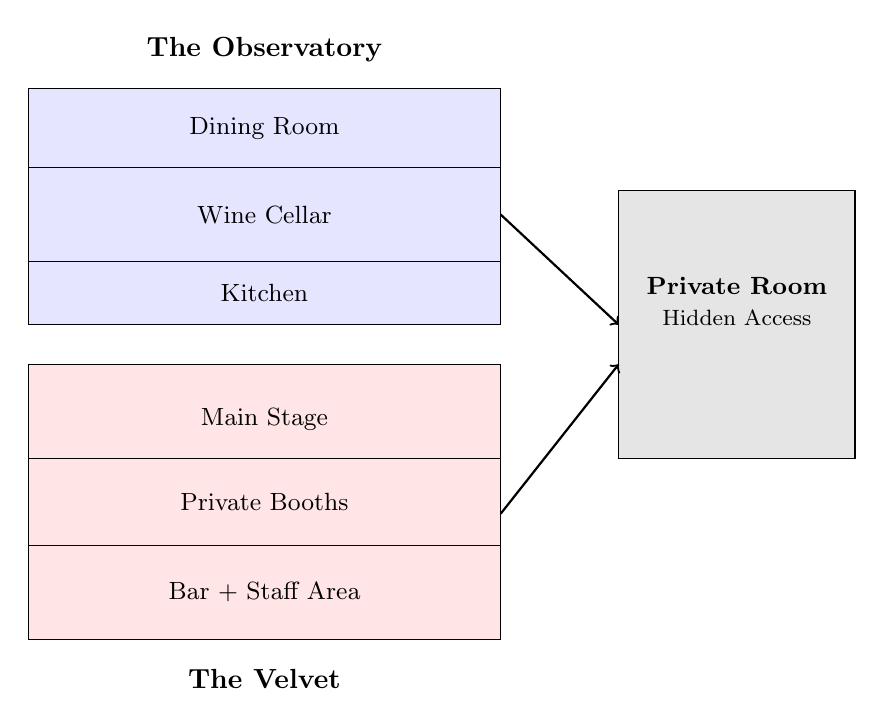
\begin{tikzpicture}[scale=1, font=\small]
  
    % === FLOOR PLAN ===
  
    % The Observatory — 1st Floor Layout
    \draw[fill=blue!10] (0,4) rectangle (6,7); % Restaurant
    \node[font=\bfseries] at (3.0, 7.5) {The Observatory};
    \draw (0,6) -- (6,6); % Divider line
    \node at (3,6.5) {Dining Room};
    \draw (0,4.8) -- (6,4.8);
    \node at (3,5.4) {Wine Cellar};
    \node at (3,4.4) {Kitchen};
  
    % The Velvet — Basement Layout
    \draw[fill=red!10] (0,0) rectangle (6,3.5); % Club
    \node[font=\bfseries] at (3,-0.5) {The Velvet};
    \draw (0,2.3) -- (6,2.3);
    \node at (3,2.8) {Main Stage};
    \draw (0,1.2) -- (6,1.2);
    \node at (3,1.75) {Private Booths};
    \node at (3,0.6) {Bar + Staff Area};
  
    % Shared Private Room
    \draw[fill=gray!20] (7.5,2.3) rectangle (10.5,5.7); 
    \node[align=center] at (9,4.3) {\textbf{Private Room}\\\footnotesize Hidden Access};
  
    % Entry arrows to Private Room
    \draw[->, thick] (6,5.4) -- (7.5,4.0); % From wine cellar
    \draw[->, thick] (6,1.6) -- (7.5,3.5); % From booths
  
    % === CORPORATE STRUCTURE ===
    %\node[font=\bfseries] at (15,8.5) {Corporate Ownership Structure};
  
    % Parent company
    %\draw[fill=black!5] (13,7.8) rectangle (17,8.3);
    %\node at (15,8.05) {\textbf{Orion Hospitality Group, LLC}};
  
    % Shells
    %\draw[fill=black!10] (13,6.8) rectangle (17,7.3);
    %\node at (15,7.05) {Shell LLC A — The Velvet};
  
    %\draw[fill=black!10] (13,5.6) rectangle (17,6.1);
    %\node at (15,5.85) {Shell LLC B — The Observatory};
  
    %\draw[fill=black!10] (13,4.4) rectangle (17,4.9);
    %\node at (15,4.65) {Shell LLC C — Private Room};
  
  \end{tikzpicture}
  \caption{
    Architectural floor plan of The Observatory (restaurant), The Velvet (club), and a hidden shared private 
    room — all legally separated by distinct shell LLCs but operated under a single parent entity.
  }
\end{figure}
  
\medskip 

The girls were not staff. But they were not exactly guests, either. The girls were just close 
enough to blur the line, and just far enough to keep anything that happened off the books.

The room itself was equal parts seduction and strategy. On the far side, a 
large circular bed 
slowly revolved under soft amber lights, not fast enough to draw attention, but just enough to suggest movement even when no 
one was on it. Opposite that, a narrow staircase led up to a small balcony lounge with low armchairs and a view that looked 
down over everything: the bed, the tables, and the guests. From up there, the whole scene played like theater.

Beneath the balcony sat a tastefully integrated dancer’s pole that was polished to a mirror finish.
Between the pole and the bed, a row of dark walnut tables offered just enough space for a whiskey flight.
Leather-backed chairs, matte black sugar trays, flickering votives completed the setup, and evoked a high-end coffee shop 
more than a club. It gave cover to whatever the guests chose to call the evening.


After dessert, it wasn’t uncommon for the night to 
migrate there.  Sometimes the wives joined. Sometimes they didn’t.  Sometimes 
they brought their own guests.  On the expense report, it was just a dinner.  It was just a networking event.  
It was just a hospitality line item.  But everyone understood. What happened in the private room wasn’t on the receipt.  
But it was part of the bargain.

If anything compromising happened in that room — a lapse in judgment, a moment of indulgence, a scene that didn’t belong 
in a compliance report — it wouldn’t trace back to the restaurant or the club. Not directly.

The layout made that possible. And so did the paperwork.

The private room acted like a firewall. It was where someone could have a ``business dinner'', and no one would ask questions. 
The circular bed wasn’t just for show, and the mirrored ceiling above it wasn’t an accident. 
Security staff knew where to turn the cameras, and the exit to the Velvet was marked only from the inside. 

\medskip

\begin{TechnicalSidebar}{Significance of a Shell LLC Leasing the Private Room}

  The decision to lease the private room under a shell company wasn’t just legal 
  hygiene. It was structural intent (Sharman, 2010).
  
  \medskip
  
  First, it created containment. If anything controversial or reputationally toxic happened behind those doors — 
  a lapse in decorum, a breach of ethics, even a crime — liability wouldn’t touch the restaurant or the club. Not 
  directly. On paper, the room belonged to a “private event services firm,” a neutral tenant with no obvious 
  connection to adult entertainment or fine dining. To regulators, auditors, or journalists, the room became a 
  dead end in the org chart (Zucman, 2015; Christensen et al., 2020).
  
  \medskip
  
  That insulation granted flexibility. The space could serve multiple roles depending on who was asking. From the 
  restaurant’s side, it might be described as a wine cellar annex or executive dining suite. From the club’s side, 
  it could be pitched as VIP overflow, though never formally listed as part of the venue. And if the conversation 
  was too delicate for either brand to claim, the room could simply be leased out to “external partners” — a 
  euphemism everyone understood (Harrington, 2016; Scott, 2009).
  
  \medskip
  
  Then came the deniability. If subpoenas arrived or FOIA requests were filed, staff could answer with complete 
  honesty: that room wasn’t under their control. Access logs, contracts, and invitations all pointed elsewhere. 
  The ambiguity wasn’t a flaw in the structure. It was the feature (Picciotto, 2007).
  
  \medskip
  
  But the real power came in access management. Because the room sat in the jurisdiction of a separate LLC, so 
  did its entry permissions. Key cards, security footage, guest lists were all handled through a different custodial 
  layer. It became a liminal space: technically private, legally detached, and socially malleable. Only insiders 
  understood how fluid the boundary really was (Levi \& Reuter, 2006).
  
  \medskip
  
  And finally, there was the financial dimension. A standalone LLC could receive funding through hospitality budgets, 
  bill clients under consulting fees, or depreciate the cost of “client engagement.” Revenues could be rerouted. 
  Expenses could be categorized to fit the desired story. And most importantly, any paper trail would read like a 
  footnote in someone else’s ledger (Desai, Dyck, \& Zingales, 2007; OECD, 2011).
  
  \medskip
  
  This wasn’t just about hiding things. It was about structuring optionality. It was not secrecy for its own sake, 
  but mobility. The kind of mobility that made denial credible, audit trails blurry, and influence hard to trace (Harvey, 2005).
  
\end{TechnicalSidebar}
  
